\section{Hacienda Consumables}
\begin{tcbraster}[raster columns=3,
	grid format]
	\tcbox[nodebox, % empty
		raster multicolumn=1,
		raster multirow=2]{}
	\tcbox[nodebox, % Schnapps
		raster multicolumn=1,
		raster multirow=2]{
		\begin{tikzpicture}
			\hacbrewnode{(0,0)}{Potato}{1}{1×1}{64}
			\hacbrewnode{(2,0)}{Schnapps}{2}
			\connect{Potato}{Schnapps}
		\end{tikzpicture}}
	\tcbox[nodebox, % Hot_sauce
		raster multicolumn=1, left=0mm, top=-7mm,
		raster multirow=2]{
	\begin{tikzpicture}
			\hacbrewnode{(0,0)}{Spices}{1}{1×1}{64}
			\hacbrewnodecons{(2.75,0)}{Hot_sauce}{2}{Jornaleros/10/4/0/2,Obreros/8.75/4/0/4,Workers/50/1/0/0,Explorers/25/3/2/0,Shepherds/100/2/0/1.5}
			\connect{Spices}{Hot_sauce}
	\end{tikzpicture}}
	\tcbox[nodebox, % Atole
		raster multicolumn=1, left=0mm,
		raster multirow=2]{
	\begin{tikzpicture}
		\hacfarmnode{(0,0)}{Sugar_cane}{1}{1×1}{64}
		\hacfarmnode{(0,-1.5)}{Corn}{2}{1×1}{64}
		\hacbrewnodecons{(2.75,-0.75)}{Atole}{2}{Obreros/8.74/4/0/16}
		\connect{Sugar_cane}{Atole}
		\connect{Corn}{Atole}
	\end{tikzpicture}}
	\tcbox[nodebox, % Rum
		raster multicolumn=1,
		raster multirow=2]{
	\begin{tikzpicture}
		\hacfarmnode{(0,0)}{Sugar_cane}{2}{1×1}{64}
		\prodnode{(0,-1.5)}{Wood}{1}{Lumberjack\%27s_Hut_(New_World)}
		\hacbrewnode{(2,-0.75)}{Rum}{2}
		\connect{Sugar_cane}{Rum}
		\connect{Wood}{Rum}
	\end{tikzpicture}}
	\tcbox[nodebox, % Atole
		raster multicolumn=1,
		raster multirow=2]{
	\begin{tikzpicture}
		\hacfarmnode{(0,0)}{Grain}{1}{1×1}{64}
		\hacfarmnode{(0,-1.5)}{Corn}{1}{1×1}{64}
		\hacbrewnode{(2,-0.75)}{Beer}{1}
		\connect{Grain}{Beer}
		\connect{Corn}{Beer}
	\end{tikzpicture}}
	\tcbox[nodebox, % Fertiliser_ratio
		raster multicolumn=1,
		raster multirow=1]{
	\begin{tikzpicture}
		\prodnode{(0,0)}{Fertiliser}{1}{Hacienda_Fertiliser_Works}
		\prodnode{(2,0)}{Silo}{10}{Fertiliser_Silo}
		\connect{Fertiliser}{Silo}
	\end{tikzpicture}}
	\tcbox[nodebox, % Fertiliser_ratio
		raster multicolumn=1,
		raster multirow=1]{
	\begin{tikzpicture}
		\prodnode{(2,0)}{Sugar_cane}{2.66}{Production_buildings}
		\prodnodelbld{(0,0)}{Sugar_cane}{1}{Production_buildings}{Silo}{\smallicon{Fertiliser}}
		\connect{Sugar_cane}{Silo}
	\end{tikzpicture}}
	\tcbox[nodebox, % Fertiliser_Works
		raster multicolumn=1,
		raster multirow=1]{
	\begin{tikzpicture}
		\prodnode{(0,0)}{Dung}{1}{Production_buildings}
		\prodnodec{(2,0)}{Fertiliser}{1}{Hacienda_Fertiliser_Works}{30}
		\connect{Dung}{Fertiliser}
	\end{tikzpicture}}
\end{tcbraster}